% This is samplepaper.tex, a sample chapter demonstrating the
% LLNCS macro package for Springer Computer Science proceedings;
% Version 2.20 of 2017/10/04
%
\documentclass[runningheads]{llncs}
%
\usepackage{graphicx}
\usepackage{enumitem}
% Used for displaying a sample figure. If possible, figure files should
% be included in EPS format.
%
% If you use the hyperref package, please uncomment the following line
% to display URLs in blue roman font according to Springer's eBook style:
% \renewcommand\UrlFont{\color{blue}\rmfamily}
\usepackage[utf8x]{inputenc}

\begin{document}

\title{LINA: A Serious Game To Help Children With Socialization Problems Using Augmented Reality\thanks{Supported by INESC-ID.}}

\titlerunning{LINA: A Serious Game}
% If the paper title is too long for the running head, you can set
% an abbreviated paper title here
%

\author{Diogo Filipe Domingos dos Santos Martins - 81983}
%
%\authorrunning{F. Author et al.}
% First names are abbreviated in the running head.
% If there are more than two authors, 'et al.' is used.
%
\institute{Orientador: João Miguel de Sousa de Assis Dias \and Departamento de Engenharia Informática \and Instituto Superior Técnico}

\maketitle              % typeset the header of the contribution

\begin{abstract}
To make socialization and interaction with peers easier for children up to pre-adolescence, especially if suffering from a diagnosed social disorder, a game with a strong social component, based on Contact Theory, is proposed. 
\par Using Augmented Reality, the targeted group of children is pitched with finding a missing colleague, searching for clues in a cooperative way, making it necessary to interact with their peers to progress further in the narrative.

\keywords{Augmented Reality \and Contact Theory \and Social Video Game.}
\end{abstract}
%
%
%

\section{INTRODUCTION}

\subsection{Motivation}

\begin{quotation}
"Man is by nature a social animal; an individual who is unsocial naturally and not accidentally is either beneath our notice or more than human. Society is something that precedes the individual. Anyone who either cannot lead the common life or is so self-sufficient as not to need to, and therefore does not partake of society, is either a beast or a god."
\end{quotation}
\par - Aristotle.
\bigskip
\par Nowadays, contact between individuals is increasingly made through digital means: Instant messengers, Voice-over-IP and video calls. Technology allows us to be closer to people, even when they are across the globe. People that do not know each other are brought closer and form social relationships thanks to that same technology. And one particular situation is the approximation of individuals through video games.
\par Quite often the public opinion about video games is slanted towards the negative side, especially among the elderly and/or conservative people, as it was, up until very recently, usually negatively portrayed in the mass media. Indeed, when a mass-shooting occurs and the shooter is a teenager, video games are quickly blamed. However, it is the failure in making the distinction between the various kinds of video games that prevent the public from fully recognizing the potential that video games present as a tool to improve some of society's problems. Even with much of the existing research focusing primarily on violence in video games, gender representation in video games, or using video games for educational purposes, there are some studies that explore the social component of video games and how can players form relationships with each other.


\subsection{Problem}
Socialization is a key process in the psychological development of a child. 
\par As the child gradually becomes a teen, his/her \textbf{social cognition} domain starts to expand and his/her awareness towards the social environment around him/her increases steadily. If asked how to describe a friend, that same description changes from physical characteristics and tastes (e.g. "he has brown hair and likes to play football") to more psychological traits, due to him/her starting to perceive the others' actions and behaviours. Also, his/her group of friends shifts from a nebulous semi-structured group of children with whom he/she can have fun and play games to a more heterogeneous and closed group of similar-minded teens that share social activities and opinions (Campos et al. 1990). 
\par As the peer-to-peer relations increase in early pre-adolescence, enthusiast, cooperative and responsive children are usually seen as the more popular in his group of people. However, a child that lacks social interactions, or that feels vulnerable by this psycho-social development and isolates himself, more often will be deem less popular and this can generate anxiety and will diminish the child's self-esteem (Tavares et al. 2007, Campos et al. 1990) creating a snowball into social alienation.
\par So, a child/pre-adolescent that has isolated himself, either by unconscious self-imposition or due to reasons external to him, has diminished social capabilities and lacks will-power and/or opportunities to engage in social activities with others.  \textbf{How can we help improve socially isolated pre-adolescents' abilities to establish successful relations with their peers?}

\subsection{Hypothesis}
  
\par There are three concept pillars used to solve the problem described above:
\begin{itemize}[noitemsep]
\item Contact Theory
\item Augmented Reality
\item User-Centered Design
\end{itemize}

\subsubsection{Contact Theory}
Hypothesized in 1954 by Gordon Allport, this notion supports that relations between distinct groups can be improved by maintaining contact in a situation that follows four rules: Equal group status in the situation; Common goals; Intergroup cooperation; Support of authorities, law or custom; (Pettigrew, 1998). Using this work hypothesis within the game, it is expected to improve the social relationships between the subjects.

\subsubsection{Augmented Reality}
Augmented Reality is not a new technology employed in the videogame industry, gaining enormous popularity with the worldwide-phenomenon that was \textit{Pokémon Go}. Tateno et al. have inclusively written about the hypothesis that the videogame could help children and teens with severe social withdrawal, although studies were not made to support the claim. 
\par \textit{Invizimals} is another interesting example of a videogame using Augmented Reality as a core feature, as it is more technologically similar to this project, using physical markers instead of geographical markers to trigger the augmented image.

\subsubsection{User-Centered Design}
As this project will be targeting pre-adolescent kids, special care must be considered when designing the concept prototype. A clean, unambiguous interface with established conventions and restricted freedom makes the users' choice-making clearer and and  However, such concept is bound to iterative revisions to improve the users' interaction.

\subsubsection{LINA}
\par Studies have shown that cooperative video games can bring families closer (Wang, Taylor \& Sun, 2018) and improve the social and affective aspects of hospitalized children by having interactions through a video game context with other children in the same condition (González et al. 2013).  
\par Interestingly, Piper et al. have also explored the possibility of developing social skills in adolescents with Asperger's Syndrome using a cooperative tabletop computer game, which is not far from the project proposed here, and have accomplished successful results with the experiment. 
%Studies (Reupert, Mayberry \& Kowalwenko, 2013) have also shown that children whose parents suffered from diagnosed mental pathologies have an increased risk of developing a mental illness themselves, and consequently suffer from decreased interaction with peers due to insufficient socialization skills. 
However, this project does not need to be restricted to these special circumstances and can be extended to all children in their pre-teens (ages 8-12) as a way to improve socialization, as it was previously shown that prosocial video games can increase prosocial behaviour to all children (Gentile et al. 2009, Griffiths, 2002).
\par In this document we present a proposal for a serious game, LINA, with a very strong social component. 
\par In LINA, a group of players, children from 8/9 to 12 years old, will attempt to find a missing colleague and her story through the discovery of hidden clues, in the form of pictures spread around the school. These pictures will be markers uncovered through augmented reality, sometimes requiring to be uncovered in pairs, which encourages the kids to interact amongst themselves to progress further in the narrative.

\section{Theorethical Background}
\subsection{Contact Theory}
\par Before Allport hypothesized the "Intergroup Contact Hypothesis" in 1954, it was believed that inter-group contact would inevitably lead to conflict, result from nineteenth century Social Darwinism, where most groups felt superior to others, naturally leading to hostility. However, no studies were conducted at that time and therefore no empirical evidence was found to support the claim. 
\par After the Second World War those suspicions changed. With the desegregation of the United States Merchant Marine in 1948, the relationship between African-American and Caucasian soldiers improved with the number of voyages taken together. Likewise, in a 1957 study by Kephart in the Philadelphia police department, the opinion of white officers regarding fellow black colleagues was more positive in subjects that previously had a black partner.
\par In 1947, Robin Williams Jr., a sociologist in the Cornell University was asked to conduct a review on intergroup relations. On his monograph \textit{The Reduction of Intergroup Tensions} he states that inter-group contact would optimally reduce prejudice under four conditions:
\begin{itemize}
    \item The two groups share similar status, interests and tasks;
    \item The situation fosters personal, intimate intergroup contact;
    \item The participants do not fit in stereotyped conceptions of their groups;
    \item The activities cut across the group lines.
\end{itemize}
\par Allport, in \textit{The Nature of Prejudice (1954)}, after extensive study, would lately adapt these four conditions into four "positive factors" that need to be present to reduce prejudice:

\begin{enumerate}
\item \textbf{Equal status between groups.} This equal status that Allport states refers \textbf{within} the situation, not \textbf{coming into}. Some writers defend that should be of equal status prior to entering the situation, but research has shown that equal status \textit{within} is enough and even more important than outside status.
\item \textbf{Common goals.} To reduce prejudice, active inter-group contact must share a common goal. By having the same objectives, the team constituents work effectively, harder and unitedly, as the different groups rely on each other, to accomplish it.
\item \textbf{Inter-group cooperation.} To work in unity towards the common goal, logically, there must not be group competition. Cooperation should be independently emphasized to each subject, as the feeling of competition undermines the effort made by the rest of the team.
\item \textbf{Support of authorities, law or custom.} With a climate of support surrounding the contact's environment, inter-group contact is more readily accepted and has more positive results. Field research in the military, business and religious institutions has emphasized the importance in support by the authority, as it is that authority that establishes the norms of acceptance.
\end{enumerate}

\par Pettigrew in his revision of the Contact Theory also proposed adding another condition onto the previous set. The condition, \textit{friendship potential} he called it, was a result of his findings where deeply prejudiced groups extremely avoid contact with each other, even when under the four conditions mentioned above. This \textit{friendship potential} condition states that "The contact situation must provide the participants with the opportunity to become friends" (Pettigrew, 1998).


\subsection{Augmented Reality}
\par A variation of Virtual Reality, but different enough to warrant a distinction, the term "Augmented Reality" has been around since the early 1990s, but the whole concept dates back to 1901 when L. Frank Baum in his short story \textit{The Master Key} described a special pair of spectacles that made the person wearing them see a letter on other people's foreheads indicating their personality (e.g. "G" for "good", "E" for "evil", etc). Then in 1968, Sutherland would revolutionize the Virtual Reality topic with the development of a "head-mounted three-dimensional display", and only twelve years later would the first wearable computer, \textit{WireTap}, be invented by Mann, where an optical display would overlay information over the image recorded by a camera. This is a natural evolution of the "heads-up display" used by the military after World War II, where HUDs based in optical reflection presented the information necessary to the pilots without blocking their view in the cockpit.
\par And it is with this last example that the distinction between \textit{Virtual Reality} and \textit{Augmented Reality} become clearer. While the former focuses on creating a separate environment from the user point-of-view, isolating him from his "real" environment, either through visual output, sounds, smells, or even tact, the last tries to enhance the current environment where the user is present, usually capturing it with a camera and overlaying it with information (e.g. text, images) but nevertheless still allowing the user to access the original information captured by his bio-sensors, i.e., eyes, ears, hence "augmenting" his senses.
\par Azuma describes Augmented Reality as systems that:
\begin{itemize}
    \item Combine real and virtual;
    \item Are interactive in real time;
    \item Are registered in 3-D;
\end{itemize}

\par AR has applications in several sectors of society:
\begin{enumerate}
    \item From a medical point-of-view it would be interesting to see and interact with a patient's MRI or CAT scan in real-time; or during a surgery, the surgeon could be accessing in real-time data about the patient or receive feedback about the procedure without having to look away from the operating table.
    \item In engineering, without having to use diagrams nor sketches, if one could see a 3D model of the artifact, the staff training would be rendered much easier. In maintenance, a description of the problem and its solution just from looking to the broken machine would be optimal in keeping minimal downtime and the costs low. 
    \item In the military, pilots have already use the precursor of this technology in their aircraft and more recently have seen it integrated with the helmets and aircraft software, and this also provides a way to soldiers receive real-time information like satellite feeds or drone reconnaissance which helps in reducing the fog-of-war.
\end{enumerate}
And of course, videogames.

\subsection{User-Centered Design}
\par User-Centered Design, is a broad term to describe design processes in which the users affect the development decisions. There are several ways the users can be involved: from requirements gathering and usability testing, to being made partners to designers through the design process.
\par The term User-Centered Design was coined by Donald Norman in his research laboratory in the University of California San Diego, but the concept was formed in his book \textit{The Psychology Of Everyday Things} (1988), where he states four rules for a design to be user-driven:
\begin{itemize}
    \item Make it easy to determine what actions are possible at any moment.
    \item Make things visible, including the conceptual model of the system, alternative actions, and the results of actions. 
    \item Make it easy to evaluate the current state of the system.
    \item Follow natural mappings between intentions and the required actions; between actions and the resulting effect; and between the information that is visible and the interpretation of the system state.
\end{itemize}
\par But just saying a design should be intuitive is not enough, so he adds seven essential design principles to facilitate the designer:
\begin{enumerate}
    \item Use both knowledge in the world and knowledge in the head. By building conceptual models, write manuals that are easily understood and that are written before the design is implemented. 
    \item Simplify the structure of tasks. Make sure not to overload the short-term memory, or the long term memory of the user.  On average the user is able to remember five things at a time. Make sure the task in consistent and provide mental aids for easy retrieval of information from long-term memory. Make sure the user has control over the task. 
    \item Make things visible: bridge the gulfs of Execution and Evaluation. The user should be able to figure out the use of an object by seeing the right buttons or devices for executing an operation.  
    \item Get the mappings right. A way to make it understandable is to use graphics. 
    \item Exploit the power of constraints, both natural and artificial, in order to give the user the feel that there is one thing to do. 
    \item Design for error. Plan for any possible error that can be made, this way the user will be allowed the option of recovery from any possible error made. 
    \item When all else fails, standardize. Create an international standard if something cannot be designed without arbitrary mappings.
\end{enumerate}
\par (Abras et al. 2004)

\newpage
\section{Related Work}

\subsection{SIDES: a cooperative tabletop computer game for social skills development}

\par The \textit{Shared Interfaces to Develop Effective Social Skills} (Piper et al. 2006), or SIDES is a tabletop computer game that aims to develop the social skills in adolescents with Asperger's Syndrome.
Based in Vygotsky's theory that learning is a social process and begins with social interaction (Vygotsky, 1978), and the supported claim that computer games help in rehabilitation for groups with special needs, and combined the two to create a collaborative activity that provided a supplement to then-current therapy techniques for teaching social and group work skills.

\subsubsection{Design Goals}
\par The objective was to develop a cooperative multiplayer tabletop computer game that encouraged group work skills like negotiation or perspective-taking for students in social group therapy, while taking into account the cognitive strengths and interests of individuals with Asperger's Syndrome.
\par After the interviews made with people suffering from Asperger's Syndrome, it was decided to create a puzzle-style game, with a theme of frogs and insects, as its visuals appealed to the interviewed individuals. 
\par SIDES is also designed to facilitate cooperative game play in a meaningful way, and to make individuals play fairly with each other.

\subsubsection{Studies and Observations}
\par The authors went to a middle school social therapy class and discussed topics with students, such as games, but also listening and leadership. 
\par They made six sessions with middle school social skills therapists and speech pathologists trying to understand teaching methods and to identify potential solutions for teaching group work skills. They have also conducted one-on-one interviews with the disorder-affected students but found that group interviews work better. 
\par In terms of results, the students complained about the current group therapy activities, and also gave the suggestion that the game should not appear too "educational", as it would make it uninteresting and not fun. With the therapists, they found that tabletop games were already used as tools during the classes, but close supervision was needed from the therapists as arguments and quarrels were frequent among the students.

\subsubsection{Game Rules}
\par The game is played by four players. At the beginning of each round, each player is given nine square tiles with arrows (three of each of three arrow types). Unique arrow types (e.g. pointing left, pointing right, around-the-corner, etc.) are distributed among the participants so that a participant cannot have all 12 arrow types in their hand. Students need to work together to build a path with their pieces to allow the frog to travel from the starting lilypad to the finishing lilypad. There is a limited supply of each arrow type, thus students are encouraged to cooperate in building an optimal path to win more points. To gain points, the path must intersect with the insect pieces on the board, each worth different points. The group must agree on one path that collects the most points with their given amount of resources. Once all players agree with the solution, the frog will travel along the path and collect points by eating all the insects in his way.

\subsubsection{Paper Prototype}
\par A paper prototype was made to finish the rules, check for game balance and whether the prototype should be turned into a digital game. It was tested with two five-student groups and the feedback was very positive, both from the students and the therapists. The students liked the theme and the game flow was suited. Therapists like how they played cooperatively and had more balanced roles instead of having dominating and least active individuals.
\par Simultaneously, they were encouraged to make a computer game as adolescents with AS are more comfortable with the controlled and structured interactions with a computer, instead of having a therapist enforcing the rules.

\subsubsection{\textit{DiamondTouch} Implementation}
\par After the paper prototype, a digital version implemented in Java for the DiamondTouch multi-user tabletop was made. The players had the same pieces and goal as the paper prototype. Each player had the arrow pieces plus three more \textit{voting buttons}: test the path, reset, or quit the game. This voting system only changes the state of the game if an option is voted unanimously, which gives the players equal status in the situation and forces the group into engaging in communication and coordination. This version did not enforce turn-taking nor piece ownership.

\subsubsection{Evaluation - Session 1}
\par In this session the research questions are:
\begin{itemize}
    \item Are tabletop computer games an appropriate and feasible tool for facilitating social skills development for this audience?
    \item Do any sensory or motor issues specific to this audience affect interaction with tabletop technology? 
\end{itemize}
\par The participants were five male students with diagnosed social disorders from the social cognitive therapy class where the paper prototype was tested. They went to the university lab to test the digital version of SIDES with their parents, per their request (the authors state that in a non-testing environment, SIDES is expected to be played while their parents are present, so it should not be a problem being so while testing).
\par In the beginning, the students were given a brief tutorial on how to use the DiamondTouch table, and proceeded to play two half-hour sessions supervised by a therapist, and after each session the therapist would convene with the group to discuss the game. The sessions were observed by two researchers and all interactions were logged by the computer.
\par The findings were positive and promising: students found SIDES to be a motivating but challenging activity. They also thought the interface was appropriate and easy to use, with much of the excitement revolved around the new technology. There were still some problems regarding the amount of control each player has, with some kids pushing each others' hands and shouting, trying to dominate and lead the others.

\subsubsection{Design Iteration}
\par SIDES was revised, now with turn-taking and controlled access (i.e. only each player can move their own pieces) to prevent other players from interfering 
with the move (as the DiamondTouch can recognize each player's input), which requires players to communicate and coordinate more.

\subsubsection{Evaluation - Session 2}
\par This session had the following guide questions:
\begin{itemize}
    \item How do students respond to computer-enforced rules versus rules provided by a human facilitator?
    \item Do any aspects of the current design encourage or discourage effective group work with this audience?
    \item What is the role of a social skills therapist during a tabletop computer activity with this special-needs population? 
\end{itemize}
\par Two groups of students were made, playing in the same environment as Session 1. The first group had played the previous iteration of the digital game, which gave them a benchmark to compare this version to, and the second group had only played the paper prototype.
\par The groups played four rounds under different conditions: Group 1: N, H, C, N and Group 2: N, C, H, N, where N = no rules, H = human-enforced rules, which means there was a therapist facilitator, and C = computer-enforced rules. Like in the first session, two observers took notes and all interactions were logged. There were also individual questionnaires and group discussion in the end.
\medskip
\par Group 1 Findings:
\par There was an increase in positive language as well as a decrease in the amount of aggressive behaviours over multiple rounds. The computer-enforced scenario was the most well performed, and the no-rules was deemed the worst in terms of team-effort. By the last round, no student touched other players' pieces nor played order-less, having adopted the turn-taking rule naturally.
\medskip
\par Group 2 Findings:
\par Contrasting to Group 1, Group 2 found the no-rule scenario the easiest of the four to work as a team. Questionnaire data supports this claim, the rule enforcing - human or computer - being the most disliked. This may be due to a particular individual that would not give up his turn, even when he had no pieces.

\subsubsection{Design Lessons}
\begin{enumerate}
\item \par Tabletop Technology as a Design Platform: the tabletop inherently provides a place for social interaction, but some students could not reach the other end of the table and the students have to be careful not to misalign the table with the ceiling projector. Tabletop computing devices should be more robust in future iterations and in further research projects.

\item Sensory and Motor Issues: the input system was appropriate as all students effectively used the interface and none presented any sensory or motor issue that prevented from playing the game.

\item Human- versus Computer-Enforced Rules: the groups in general responded better to computer-enforced rules as it is less subjective than the input from a human, and in their minds, more impersonal and trustworthy.

\item Embedded Structure: the voting buttons encouraged the users to cooperate and discuss and reach a consensus to progress in the game. Piece ownership balanced the roles of the players by not defining a leader \textit{ab initio}. Computer-enforced turn-taking combined with piece ownership worked for one group but not for the other as mentioned above. In future iterations maybe a hybrid human/computer approach would prevent these situations.

\item Need for an Adult Moderator: as SIDES was not made as a standalone tool, the presence of the students' therapist is crucial to the experience, as this authority helps them consolidating the abstract topics into shared real experience, and controls the behaviours during the group work sessions.

\item Challenges in Participatory Design: due to the special needs of its users, the authors needed extensive preparation in advance, such as lengthy contact with the parents and therapists, encouraging them to participate in the sessions. Sometimes, the students scheduled for an individual interview would "shut down" and no longer answer the questions, which made the authors switch to group interviews.
\end{enumerate}

\subsubsection{Discussion, Impact \& Conclusion}
\par SIDES gives students an engaging experience where they can develop their social skills and group work, that otherwise would be a challenging situation. In the game, they made an effort to collaborate and communicate with their peers, which is remarkable as they promptly disengage when unmotivated or uninterested in a task.
\par The authors underline the importance and potential of supportive social entertainment programs through the tabletop technology in dealing with issues amongst a population with special needs. More than that, they stress that the game works because, is not only educational in terms of group work, but also does not appear to be so, which makes it more fun and appealing. Therapists also mentioned how it evens out the class: the more quiet and isolated are "given a louder voice", while the more outspoken and dominating become more restrained in their interventions.
\par This article sets the ground work for future research in using tabletop technology and user-centered design regarding the special needs of this population, as well as games that aim to facilitate social interaction and group work skills. 

\subsection{Pathomon: A Social Augmented Reality Serious Game}
\par Pathomon takes the premise created by the blockbuster \textit{Pokémon GO} and turns it into a serious game designed to make the players aware of the known viruses and how to eradicate them while being a social experience.
\subsubsection{Concept}
\begin{enumerate}
    \item \textbf{The Story.} The player dives into the journey of a young scientist tasked with eradicating viruses.
    \item \textbf{Game Procedures.} Players have to find QR codes, corresponding to antidote ingredients or viruses, in an area. By collecting the ingredients, they can craft antidotes, which then can be used to attack viruses. These actions give the player experience points. Some viruses need to be attacked by more than one player. This, along with having to share the QR codes' locations and the right combination of ingredients to make the antidotes with the other players, gives the game a strong social component.
    \item \textbf{Mechanics.} The player creates a personal account, and then is given a profile of an expert on a certain virus. This means that they can "contaminate" certain QR codes the player has interacted with. This profile also records the player level, his achievements and the global score ladder. The players can level up with the earned experience points, unlocking new viruses and antidotes. The \textit{Pathodex} and \textit{Inventory} records the fought viruses and stores the antidotes, respectively.
    \item \textbf{Conveying Knowledge} Throughout the game, facts about the viruses are unlocked, like size, lethality, symptoms, incubation time, method of transmission, etc. Some "fun facts" are also stated. Realistic shapes are used for the viruses' appearance in the AR part of the game.
\end{enumerate}

\subsubsection{Implementation}
\par The game was made in Unity3D to achieve multi-platform support. For AR, Kudan platform was used. An Amazon AWS EC2 instance attached to an Amazon RDS database hosts the server-side implementation and API. \textit{Pathomon} can be played in iOS and Android devices.

\subsubsection{User Study}
\par A study conducted during the 2017 International Genetically Engineered Machine (iGEM) Conference, in which attending people were asked to play the game, revealed that sensory immersion and positive affect were praised, but the game flow and challenge were only reasonable, as they felt the game start and progress too difficult. In the social aspect, the interviewed people did not think their actions could affect the actions of the others, maybe be due to focusing on their own progress. However, this study was made in a poorly controlled environment and with a very low number of subjects, so a follow up study was proposed by the authors to eliminate unreliable results.

\subsubsection{Discussion and Conclusion}
\par The user study revealed positive opinions about the game, but still has room for improvement, like the progress and flow.
\par Although the game is used for giving knowledge about viruses, its mechanics could be used in various other contexts. A possible step in the future is the further development towards a versatile platform whose content for learning can be easily swapped. 



\subsection{Development of a Videogame to Improve Communication in Children with Autism}
\par This article refers to the development of a videogame made to improve the communication of children with autism, on the basis that videogames can positively change an ASD-affected child's social behaviour towards other children.

\subsubsection{Designing the Content}
\par The authors met with experts on autism to understand what made the children isolate themselves and what techniques and methods were better suited to design an effective tool in complementing the conventional therapy, using the \textit{Theacch, Treatment and Education of Autistic and Related Communication-Handicapped Children}, method.
\par The objective is to improve social interaction by showing a pictogram with basic activities that can be performed in school or at home.
The game's complexity can be changed to adapt to the child's preferences, hence the content shown can change (from a pictogram to images to categories). An important aspect is the positive reinforcement through points and trophies rewarded, promoting motivation to learn and social engagement.

\subsubsection{Designing the Game and its Progress}
\par The game design follows the iterative model. Developed in Unity3D for the multi-platform mobile support plus the the ability to be played in a webpage through Unity Web Player.
\par The game takes place in a nature-laden scenery, with the purpose to raise awareness in the child that he is part of an environment and his actions are part of said environment. It focuses on the development of communication and learning abilities through the visual interface and interaction, so that the kid feels compelled into finishing all activities within the game.

\subsubsection{Description of the Game}
\par The game provides a fun and friendly environment to improve the verbal and non-verbal communication. The game is split into two sections: the \textit{communication panel} and \textit{knowing animals, places and ecosystems}.
\par The communication section shows a thematic panel related with the place or activity. The interface is composed of a group of pictograms of basic activities that can be performed at home or in school. The game allows to eliminate or add images to customize the panel to each individual according to his needs. Through this panel the child can associate meanings to each image, allowing him to express his thoughts and emotions. In the bottom portion of the screen there is a board where he can construct a phrase through the combination of pictures.
\par The \textit{knowing animals} section is made of two modes: Learn and Play.
\paragraph{Learn Mode} This mode shows several animals through a name, a real-life picture, a caricature, and with the click of a button, the sound they make.
\paragraph{Play Mode} In this section the child demonstrates his knowledge about the animals from the previous mode. The picture and caricature of a randomly selected animal appears, and from three different options its name must be chosen. In case of answering incorrectly the game gives another chance, hence the child always ends up choosing the right answer. Upon choosing the right answer points are awarded.

\subsubsection{Conclusion}
\par Videogames have been shown as successful tools for learning, both technical and social skills. The developed videogame has been positively evaluated by therapists and experts in autistic disorders, and interest has been shown by ASD-affected children, but no studies were conducted. As future work, the game could be incorporated in conventional therapy to study and evaluate the usefulness of this tool as a way to improve the communication and social interaction skills.

\subsection{Design Pattern Canvas: Towards Co-Creation of Unified Serious Game Design Patterns} 
\par Motivated by the lack of a standardized approach on designing serious games, this article proposes an alpha version based on Osterwalder's Business Model Canvas.
\subsubsection{Game Design Patterns for Serious Games}
\paragraph{What Are Game Design Patterns?} A design pattern is a solution that can be reused to solve recurring problems, and is described as causes and effects to reach an objective. Not all design aspects are problem solving, especially in game design.
\paragraph{Why Use Patterns for Serious Games Design?} Game design patterns are useful for problem-solving during development as a creative design tool and communication facilitator between peers and professions. Patterns also help to better understand game features and can be used to evaluate design problems, especially in experimental game design.
\paragraph{Criticism of Patterns} Usually patterns are criticized as either too formal or not formal enough, not only in game design, but also in other fields. However, the criticism draws from the quality of their conceptualization, rather than the notion itself, and the fact that patterns are only useful for solving specific problems within the application development.

\subsubsection{Design Pattern Canvas}
\par There are a set of considerations when designing the canvas as to not sacrifice freedom and creativity when designing the experimental prototype. As such the canvas should be:
\begin{itemize}
    \item Intuitive and familiar;
    \item Easy to update and enabling iterations;
    \item Not time consuming to create;
    \item Short (preferably fit on a single page);
    \item Using a widely shared design language;
    \item Facilitating knowledge sharing and transfer;
    \item A Tool to build experimental prototypes directly from the definition of a set of game characteristics;
    \item Standardized;
    \item Considering the perspectives of designer and player;
\end{itemize}

The Design Pattern Canvas (fig.\ref{fig:DPC}) helps to break larger problems into smaller ones and assists in a bottom up approach in designing serious games.
\par The descriptions are not supposed to contain all the information and should be complemented with diagrams. The chart can be split into two sections: the left is associated with design questions and the right is focused on interaction design.

\subsubsection{Discussion \& Conclusion}
\par The Design Pattern Canvas is admittedly still in an infant stage and many questions shall be addressed in future development.
\begin{figure}
    \centering
    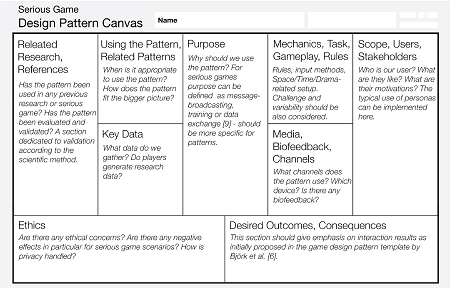
\includegraphics{Screenshot_20.png}
    \caption{Design Pattern Canvas}
    \label{fig:DPC}
\end{figure}

\subsection{Robotic gaming companion to facilitate social interaction among children}
\par By using a robot that displays human actions like cheering and crying when playing a videogame, this article suggests that children can improve their interaction with robots and humans alike.

\subsubsection{Introduction}
\par Problems in socializing have been proven to be reduced through rehabilitation of human-to-human interaction, and one of the approaches used in literature is through a robot, like Kojima's Keepon to encourage interaction in autistic children, as they show an interest towards robots that is not shown towards people.
\par A novel human-robot interaction approach is proposed, to encourage interaction, with the children playing videogames with a robot. 
\par Two research questions are placed:
\begin{enumerate}
    \item How can a robotic gaming companion facilitate human-robot interaction?
    \item How can a robotic gaming companion facilitate human-human interaction?
\end{enumerate}
\par Videogames are a common medium through which children communicate, plus is fun and engaging. The authors believe that a robotic companion can act as a facilitator in interaction among children playing videogames.

\subsubsection{Approach}
\par Communication during gaming can be seen from several perspectives: as cooperative or competitive among players, as between players and audience, and occurring before, during and after gaming.
\par A robot that is able of playing videogames like a human is expected to communicate with those humans. Hence, two factors are studied: playability, i.e. the ability to retain people's attention without natural expressions, and communicability, i.e. the ability to encourage interaction without unnatural expressions. Previous studies stated unnatural expressions should be removed from gaming communication as it affects people's behaviour and ruins the benefits of gaming.
\par The robot must be humanoid and perform similarly to, if not better than, a human, such as it presents a challenge but does not lead to player frustration, nor boredom.

\subsubsection{System Overview}
\par Aldebaran Robotics humanoid robot \textit{NAO} was chosen to play Wii videogames (chosen for their strong familiar and social component, bigger than most games in the industry), in particular \textit{Taiko no Tatsujin}, a music video game where the objective is to hit a drum-like controller in the rim or at the center synchronized with the song playing. Score is given by how closely the hits were with the symbols on-screen, much like \textit{Guitar Hero} or \textit{Band Hero}.

\subsubsection{Methodology}
\par The game sends an HDMI signal that is split into a computer and a monitor. The signal sent to the computer is then processed and the resulting action sent to the robot. The robot is controlled by two methods: autonomous game play and the Wizard of Oz framework, the last for a smooth and natural interaction with humans.
\paragraph{Autonomous Game Play} The image received is processed for locating the colors associated with the symbols (red for the center, blue for the rim, orange for the face repeatedly) and calculates the distance and temporal difference from the image's edge until the hit mark, so that calculations are made to know precisely when to hit the \textit{taiko} according to the song's beats per minute.
\paragraph{WOZ Framework} A doll-type interface was used to wirelessly control the entire body in real time. This allows the user to control the robot by changing the doll's posture. High-level commands like sitting and greeting can be stored and triggered with buttons.

\subsubsection{Interaction Scenarios}
\par The robot is capable of three types of interaction: greeting, expression and facilitation. The greeting is executed verbally with a "hello", for example. Expression behaviour are for after gaming, like a "Banzai" when it wins a game, or "Anger" for when it loses. Facilitation is used when cheering for a player or booing an opponent.
\par There are three phases for the interaction: preparation, game and expression. First, in preparation, the robot is assigned as a player or an audience member. As such it performs the appropriate behavior like a handshake or a greeting. In the game phase, it either cheers for a player, or plays the game. In the expression phase, according to the result, the robot shows its feelings, such as "win pose" or "crying".

\subsubsection{Experiment}
\par First an experiment was conducted to see if the robot's performance in-game was similar to a human. After a successful result, a study with children was conducted. The doll operator was out of the child's sight. The robot performed the greeting motion when the participant entered by saying hello, gazing at him, and encouraging him to play the game. During the game phase the robot played autonomously. In the third phase the robot performed their positive or negative behaviour according to the result.
\par The participant's behaviour throughout the experiment was analyzed and found that during the game his interactions rarely occurred during the game phase, perhaps due to be concentrated in the game. However, during the preparation and expression phases the social interactions were recurring.

\subsubsection{Conclusion}
\par The robot introduced has shown that was able to play like a human, and in the preliminary study, it was capable of playing a videogame with children and facilitate human interaction.
\par In future research, interaction between the human and the robot in a cooperative setting will be investigated. The playing algorithm will also be tuned. Also, a feasibility test will be conducted with hospitalized children, or autistic children in therapy, with the purpose to use the robot-assisted activities to improve social interaction amongst these children.


\subsection{Implementation of an chatbot in a serious game associated with the acquisition of social skills and the promotion of collaborative tasks in children}

\subsubsection{Introduction}
\subsubsection{Background}
\subsubsection{Prototype Proposed}
\subsubsection{Discussion and Future Work}


\subsection{Tabletop Prototyping of Serious Games for 'Soft Skills' Training}

\subsubsection{Introduction}
\subsubsection{Background}
\subsubsection{A Board Game Prototype for Soft Skills Training}
\subsubsection{Conclusions and Future Work}

\subsection{An adoption framework for mobile augmented reality games: The case of Pokémon Go}

\section{Implementation}
\section{Evaluation}
\section{Conclusion}


Table~\ref{tab1} gives a summary of all heading levels.

\begin{table}
\caption{Table captions should be placed above the
tables.}\label{tab1}
\begin{tabular}{|l|l|l|}
\hline
Heading level &  Example & Font size and style\\
\hline
Title (centered) &  {\Large\bfseries Lecture Notes} & 14 point, bold\\
1st-level heading &  {\large\bfseries 1 Introduction} & 12 point, bold\\
2nd-level heading & {\bfseries 2.1 Printing Area} & 10 point, bold\\
3rd-level heading & {\bfseries Run-in Heading in Bold.} Text follows & 10 point, bold\\
4th-level heading & {\itshape Lowest Level Heading.} Text follows & 10 point, italic\\
\hline
\end{tabular}
\end{table}


\noindent Displayed equations are centered and set on a separate
line.
\begin{equation}
x + y = z
\end{equation}

\begin{theorem}
This is a sample theorem. The run-in heading is set in bold, while
the following text appears in italics. Definitions, lemmas,
propositions, and corollaries are styled the same way.
\end{theorem}
%
% the environments 'definition', 'lemma', 'proposition', 'corollary',
% 'remark', and 'example' are defined in the LLNCS documentclass as well.
%
\begin{proof}
Proofs, examples, and remarks have the initial word in italics,
while the following text appears in normal font.
\end{proof}
For citations of references, we prefer the use of square brackets
and consecutive numbers. Citations using labels or the author/year
convention are also acceptable. The following bibliography provides
a sample reference list with entries for journal
articles~\cite{ref_article1}, an LNCS chapter~\cite{ref_lncs1}, a
book~\cite{ref_book1}, proceedings without editors~\cite{ref_proc1},
and a homepage~\cite{ref_url1}. Multiple citations are grouped
\cite{ref_article1,ref_lncs1,ref_book1},
\cite{ref_article1,ref_book1,ref_proc1,ref_url1}.
%
% ---- Bibliography ----
%
% BibTeX users should specify bibliography style 'splncs04'.
% References will then be sorted and formatted in the correct style.
%
% \bibliographystyle{splncs04}
% \bibliography{mybibliography}
%
\begin{thebibliography}{8}

\bibitem{ref_article1}   \textbf{Wang, B., Taylor, L., \& Sun, Q.} (2018). Families that play together stay together: Investigating family bonding through video games. New Media \& Society, 20(11), 4074–4094. \doi{10.1177/1461444818767667}

\bibitem{ref_article2} \textbf{González, C.S., Toledo, P., Collazos, C.A., \& González-Sanchez, J.L.} (2013). Design and analysis of collaborative interactions in social educational videogames. Computers in Human Behavior 31 (2014) 602–611. \doi{10.1016/j.chb.2013.06.039}

%\bibitem{ref_article3} \textbf{Reupert, A.E., Maybery, D.J, \& Kowalenko, N.M.} (2013). Children whose parents have a mental illness: prevalence, need and treatment. Medical Journal of Australia 2013; 199 (3 Suppl): S7-S9. \doi{10.5694/mja11.11200}

\bibitem{ref_proc1} \textbf{Piper, A.M, O'Brien, E., Morris, M.R., \& Winograd, T.} (2006). SIDES: a cooperative tabletop computer game for social skills development. In: Proceedings of the 2006 20th anniversary conference on Computer supported cooperative work, November 04-08, 2006, Banff, Alberta, Canada. \doi{10.1145/1180875.1180877}

\bibitem{ref_article4} \textbf{Gentile, D. A., et al.} (2009) The Effects of Prosocial Video Games on Prosocial Behaviors: International Evidence From Correlational, Longitudinal, and Experimental Studies. Personality and Social Psychology Bulletin, vol. 35, no. 6, June 2009, pp. 752–763. \doi{10.1177/0146167209333045}

\bibitem{ref_article5} \textbf{Griffiths, M.D.} (2002) The educational benefits of videogames. Education and Health, 20(3), 47–51.

\bibitem{ref_book1} \textbf{Campos, B.P., Ribeiro, J.L.P., Fontaine, A.M., Ribeiro, A., Taveira, M.C.} Psicologia do Desenvolvimento e Educação de Jovens vol.II. Universidade Aberta, Lisboa (1990) 

\bibitem{ref_book2} \textbf{Tavares, J., Pereira, A.S., Gomes, A.A., Monteiro, S.M., Gomes, A.} Manual de Psicologia do Desenvolvimento e Aprendizagem. Porto Editora, Porto (2007)

\bibitem{ref_article6} 	\textbf{Tateno, M., Skokauskas, N., Kato, T. A., Teo, A. R., \& Guerrero, A.} (2016). New game software (Pokémon Go) may help youth with severe social withdrawal, hikikomori. Psychiatry research, 246, 848-849. \doi{10.1016/j.psychres.2016.10.038}

\bibitem{ref_article7} \textbf{Kato, T.A., Teo, A.R., Tateno, M., Watabe, M., Kubo, H. \& Kanba, S.} (2017), Can Pokémon GO rescue shut-ins (hikikomori) from their isolated world?. Psychiatry Clin. Neurosci., 71: 75-76. \doi{10.1111/pcn.12481}

\bibitem{ref_article8} \textbf{Pettigrew, T.F.} (1998). INTERGROUP CONTACT THEORY. Annual Review of Psychology, 49(1), 65–85. \doi{10.1146/annurev.psych.49.1.65}

\bibitem{ref_proc2} \textbf{Sutherland, I.E.} (1968). A head-mounted three dimensional display. Proceedings of the December 9-11, 1968, Fall Joint Computer Conference, Part I on - AFIPS ’68 (Fall, Part I). \doi{10.1145/1476589.1476686}

\bibitem{ref_article9} \textbf{Azuma, R.T.} (1997) A Survey of Augmented Reality
Presence: Teleoperators and Virtual Environments 1997 Vol.6, Issue 4, 355-385 \doi{10.1162/pres.1997.6.4.355}

\bibitem{ref_book3} \textbf{Vygotsky,  L.S.} (1978).  Mind in Society: The development of higher  psychological  processes.  Harvard University Press (1980). 

\bibitem{ref_article9} \textbf{Rapp, D., Müller, J., Bucher, K., \& Von Mammen, S.} (2018) Pathomon: A Social Augmented Reality Serious Game, 2018 10th International Conference on Virtual Worlds and Games for Serious Applications (VS-Games), Wurzburg, 2018, pp. 1-4. \doi{10.1109/VS-Games.2018.8493437}

\bibitem{ref_article10} \textbf{Bringas, J.A.S., Léon, M.A.C., Cota, I.E., and Carrillo, A.L.} (2016) Development of a videogame to improve communication in children with autism, 2016 XI Latin American Conference on Learning Objects and Technology, San Carlos, 2016, pp. 1-6. \doi{10.1109/LACLO.2016.7751751}

\bibitem{ref_article11} \textbf{Zavcer, G., Mayr, S., \& Petta, P.} (2014) Design Pattern Canvas: Towards Co-Creation of Unified Serious Game Design Patterns, 2014 6th International Conference on Games and Virtual Worlds for Serious Applications (VS-GAMES), Valletta, 2014, pp. 1-2.
\doi{10.1109/VS-Games.2014.7012153}

\bibitem{ref_article12} \textbf{Hirose, J., Hirokawa, M., \& Suzuki, K.} (2014) Robotic gaming companion to facilitate social interaction among children, The 23rd IEEE International Symposium on Robot and Human Interactive Communication, Edinburgh, 2014, pp. 63-68. \doi{10.1109/ROMAN.2014.6926231}

\bibitem{ref_article13} \textbf{Mansilla, A., Ochoa, A., Ponce, J., Herrera, M., Hernández, A., \& Cossio, E.} (2017) "Implementation of an chatbot in a serious game associated with the acquisition of social skills and the promotion of collaborative tasks in children," 2017 Twelfth Latin American Conference on Learning Technologies (LACLO), La Plata, 2017, pp. 1-4.
\doi{10.1109/LACLO.2017.8120912}

\bibitem{ref_article14} \textbf{Abras, C., Maloney-Krichmar, D., \& Preece, J.} (2004). User-centered design. Bainbridge, W. Encyclopedia of Human-Computer Interaction. Thousand Oaks: Sage Publications, 37(4), 445-456.

\bibitem{ref_lncs0}
Author, F., Author, S.: Title of a proceedings paper. In: Editor,
F., Editor, S. (eds.) CONFERENCE 2016, LNCS, vol. 9999, pp. 1--13.
Springer, Heidelberg (2016). \doi{10.10007/1234567890}

\bibitem{ref_article0}
Author, F.: Article title. Journal \textbf{2}(5), 99--110 (2016)

\bibitem{ref_book0}
Author, F., Author, S., Author, T.: Book title. 2nd edn. Publisher,
Location (1999)

\bibitem{ref_proc0}
Author, A.-B.: Contribution title. In: 9th International Proceedings
on Proceedings, pp. 1--2. Publisher, Location (2010)

\bibitem{ref_url0}
LNCS Homepage, \url{http://www.springer.com/lncs}. Last accessed 4
Oct 2017
\end{thebibliography}
\end{document}
